\documentclass[aspectratio=169,10pt]{beamer}

\usepackage[utf8]{inputenc}
\usepackage[T1]{fontenc}
\usepackage[shorthands=off, turkish]{babel}
\usepackage{amsmath,amssymb,amsfonts}
\usepackage{graphicx}
\graphicspath{{figures/}{./}}
\usepackage{booktabs}
\usepackage{tabularx}
\usepackage{array}

% --- IEEE Conference Presentation Theme & Colors ---
\usetheme{Madrid}
\usecolortheme{whale}
\definecolor{IEEEBlue}{RGB}{0, 98, 155}
\definecolor{IEEENavy}{RGB}{0, 40, 85}
\definecolor{IEEEGray}{RGB}{242, 245, 248}

\setbeamercolor{palette primary}{bg=IEEENavy,fg=white}
\setbeamercolor{palette secondary}{bg=IEEEBlue,fg=white}
\setbeamercolor{palette tertiary}{bg=IEEENavy,fg=white}
\setbeamercolor{structure}{fg=IEEEBlue}
\setbeamercolor{title}{bg=IEEENavy,fg=white}
\setbeamercolor{frametitle}{bg=IEEENavy,fg=white}
\setbeamercolor{block title}{bg=IEEEBlue,fg=white}
\setbeamercolor{block body}{bg=IEEEGray,fg=black}
\setbeamertemplate{navigation symbols}{}
\setbeamertemplate{caption}[numbered]

\title[IEEE Final Sunum --- Deep Learning]{Önceden Eğitilmiş Türkçe Modellerle İnce Ayar (Fine-Tuning) Tabanlı Chatbot Geliştirme ve Seq2Seq Karşılaştırmalı Başarım Analizi}
\subtitle{Nihai Proje Sunumu (Final Presentation) --- IEEE Akademik Formatı}
\author[Seyit Ali Arslan (240711024)]{\textbf{Seyit Ali Arslan} \\ Öğrenci No: 240711024}
\institute[Atatürk Üniversitesi]{Yapay Zeka ve Veri Mühendisliği Bölümü\\Atatürk Üniversitesi, Erzurum, Türkiye\\Ders: Deep Learning (2026--2027)}
\date{Kasım 2026}

\begin{document}

% --- SLAYT 1: Kapak ---
\begin{frame}
    \titlepage
\end{frame}

% --- SLAYT 2: Sunum Akışı ---
\begin{frame}{Sunum Akışı (IEEE Bölümlendirmesi)}
    \begin{columns}[T]
        \begin{column}{0.48\textwidth}
            \begin{block}{I--IV. Teorik Çerçeve, Veri ve Metodoloji}
                \begin{itemize}
                    \item \textbf{I. Giriş ve Problem Tanımı:} Sondan eklemeli Türkçe morfolojisi ve Seq2Seq darboğazı
                    \item \textbf{II. Motivasyon:} Sıfırdan Eğitim vs. Transfer Öğrenme (Full FT \& LoRA)
                    \item \textbf{III. Veri Kümesi ve EDA:} 50.000 Türkçe Diyalog Çifti (\%80 / \%10 / \%10)
                    \item \textbf{IV. Metodoloji:} BPE Tokenizasyon, Causal Self-Attention ve LoRA ($\Delta W = BA$)
                \end{itemize}
            \end{block}
        \end{column}
        \begin{column}{0.48\textwidth}
            \begin{block}{V--VIII. 3 Modelin Karşılaştırmalı Analizi}
                \begin{itemize}
                    \item \textbf{V. Eğitilen 3 Model:} Baseline Bi-LSTM vs. Model 1 (Full FT) vs. Model 2 (LoRA / PEFT)
                    \item \textbf{VI. Deneysel Sonuçlar:} Loss, Perplexity (PPL), BLEU-1/2, ROUGE-1/L ve Latency (ms)
                    \item \textbf{VII. Niteliksel (Human Evaluation) Analiz:} Akıcılık, Tutarlılık ve Örnek Diyaloglar
                    \item \textbf{VIII. Canlı Web Arayüzü (\texttt{app\_web.py}) \& Sonuç}
                \end{itemize}
            \end{block}
        \end{column}
    \end{columns}
\end{frame}

% --- SLAYT 3: Giriş, Problem Tanımı ve Motivasyon ---
\begin{frame}{I. Giriş ve Problem Tanımı \& II. Motivasyon}
    \begin{columns}[T]
        \begin{column}{0.48\textwidth}
            \begin{block}{I. Problem Tanımı}
                \begin{itemize}
                    \item \textbf{Sondan Eklemeli (Agglutinative) Yapı:} Türkçede kök + yapım/çekim ekleri kelime dağarcığını üstel büyütür ve \textbf{OOV (Out-of-Vocabulary)} sorununa yol açar.
                    \item \textbf{Seq2Seq RNN/LSTM Sınırları:} Sıralı (\textit{sequential}) işleme nedeniyle uzun cümlelerde \textbf{darboğaz (bottleneck)} ve bağlam kaybı yaşanır.
                \end{itemize}
            \end{block}
        \end{column}
        \begin{column}{0.48\textwidth}
            \begin{block}{II. Motivasyon ve 3'lü Kıyaslama}
                \begin{itemize}
                    \item \textbf{Transfer Öğrenme:} Genel Türkçe metinlerde eğitilmiş \texttt{Turkish-GPT-2} ağırlıklarını diyalog verisine aktarmak.
                    \item \textbf{3 Mimari Kıyaslaması:}
                    \begin{enumerate}
                        \item \textbf{Baseline:} 2-Katmanlı Seq2Seq Bi-LSTM + Attention (Sıfırdan, 23.1M)
                        \item \textbf{Model 1:} Full Fine-Tuned GPT-2 (124.4M, \%100)
                        \item \textbf{Model 2:} LoRA / PEFT GPT-2 (1.62M, \%1.29)
                    \end{enumerate}
                \end{itemize}
            \end{block}
        \end{column}
    \end{columns}
\end{frame}

% --- SLAYT 4: Veri Kümesi ve Bölümleme ---
\begin{frame}{III. Veri Kümesi ve Veri Bölümleme (\%80 / \%10 / \%10)}
    \begin{columns}[c]
        \begin{column}{0.44\textwidth}
            \begin{block}{Veri Önişleme Boru Hattı}
                \begin{itemize}
                    \item \textbf{Kaynaklar:} Hugging Face Türkçe diyalog kümeleri (\texttt{Ba2han/Turkish\_Chat}, \texttt{AEG/Turkish-Chat-62k}, \texttt{yeniguno/turkish-chatbot-data}).
                    \item \textbf{Temizleme:} HTML, Markdown kalıntıları, bozuk karakterler ve mükerrer kayıtlar elendi.
                    \item \textbf{Toplam Boyut:} \textbf{50.000} filtrelenmiş doğal Türkçe diyalog çifti (2--45 kelime).
                    \item \textbf{Bölümleme:} \textbf{40.000} Train (\%80), \textbf{5.000} Val (\%10), \textbf{5.000} Test (\%10).
                \end{itemize}
            \end{block}
        \end{column}
        \begin{column}{0.54\textwidth}
            \centering
            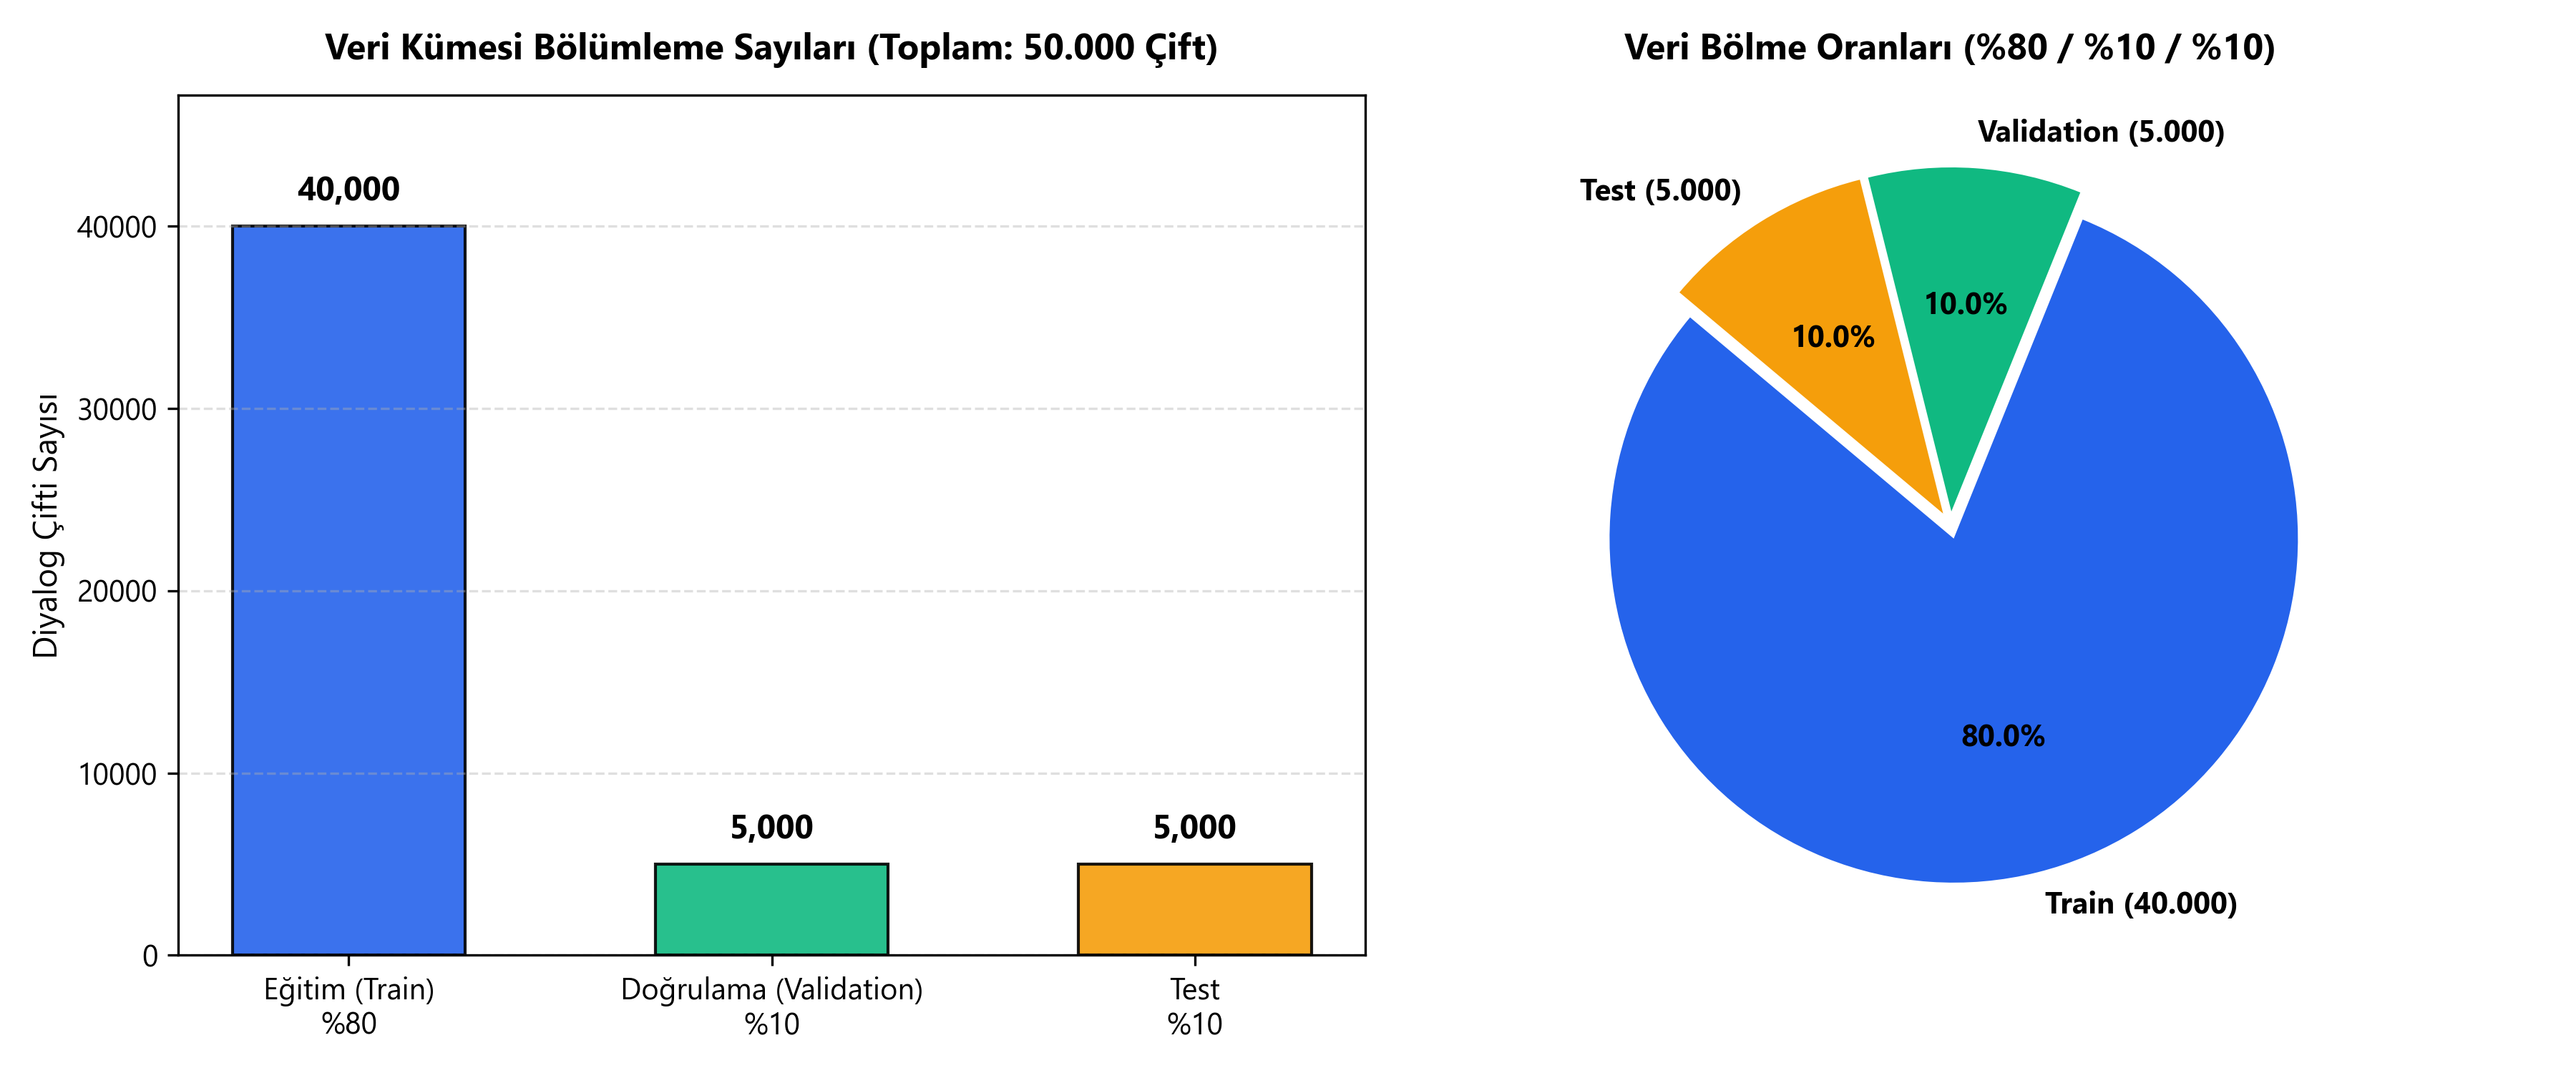
\includegraphics[width=0.98\textwidth]{01_veri_bolumleme_split.png}
        \end{column}
    \end{columns}
\end{frame}

% --- SLAYT 5: Keşifsel Veri Analizi (EDA) ---
\begin{frame}{III. Keşifsel Veri Analizi (EDA): Uzunluk ve Kaynak Dağılımı}
    \begin{columns}[c]
        \begin{column}{0.52\textwidth}
            \centering
            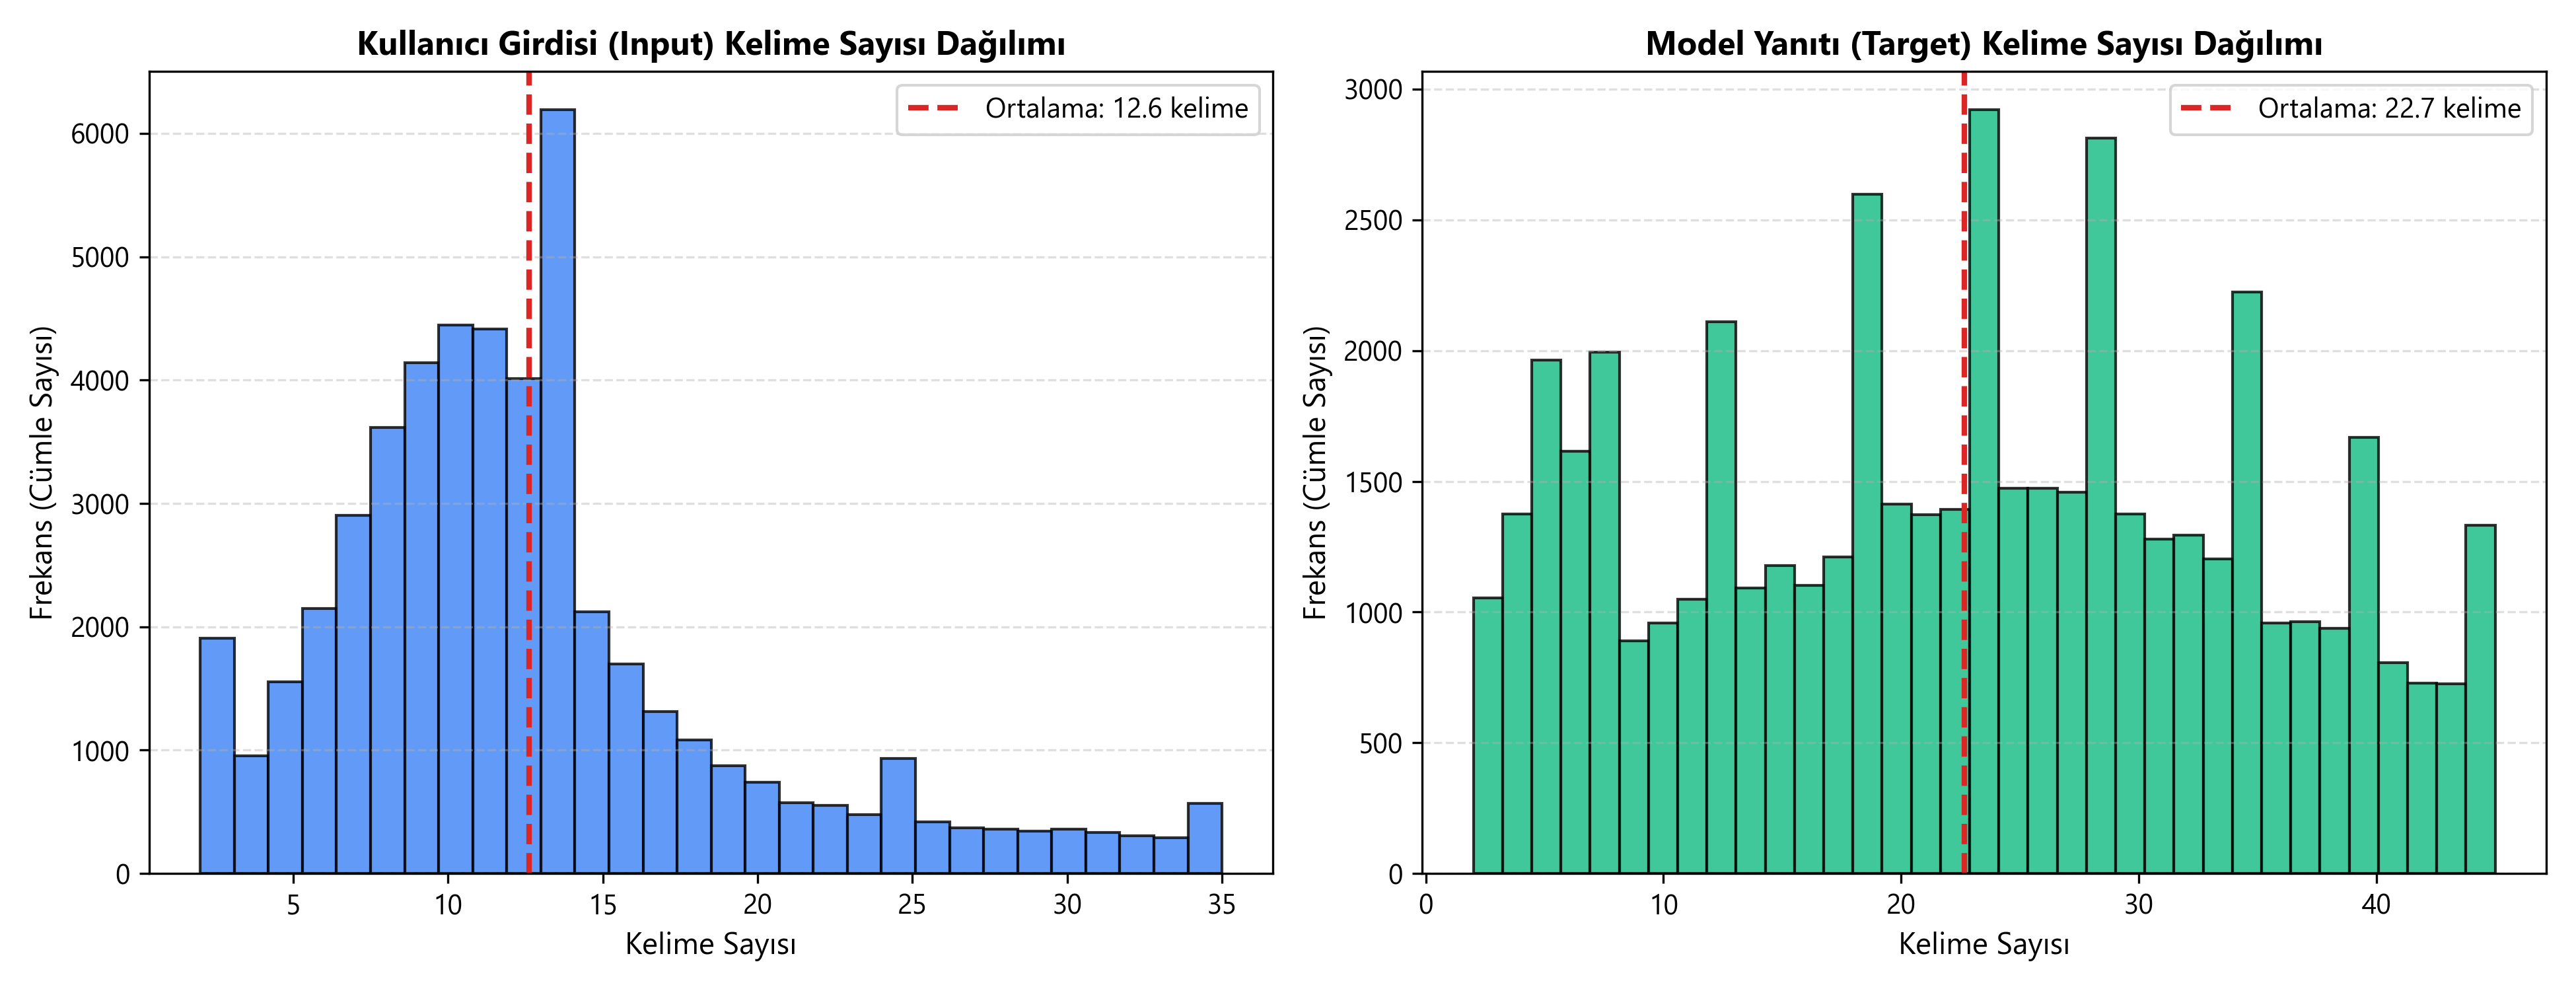
\includegraphics[width=0.98\textwidth]{02_kelime_uzunlugu_dagilimi.png}
            \vspace{2pt}
            {\scriptsize Ortalama Girdi: \textbf{9.73 kelime} $\mid$ Ortalama Yanıt: \textbf{15.49 kelime}}
        \end{column}
        \begin{column}{0.46\textwidth}
            \centering
            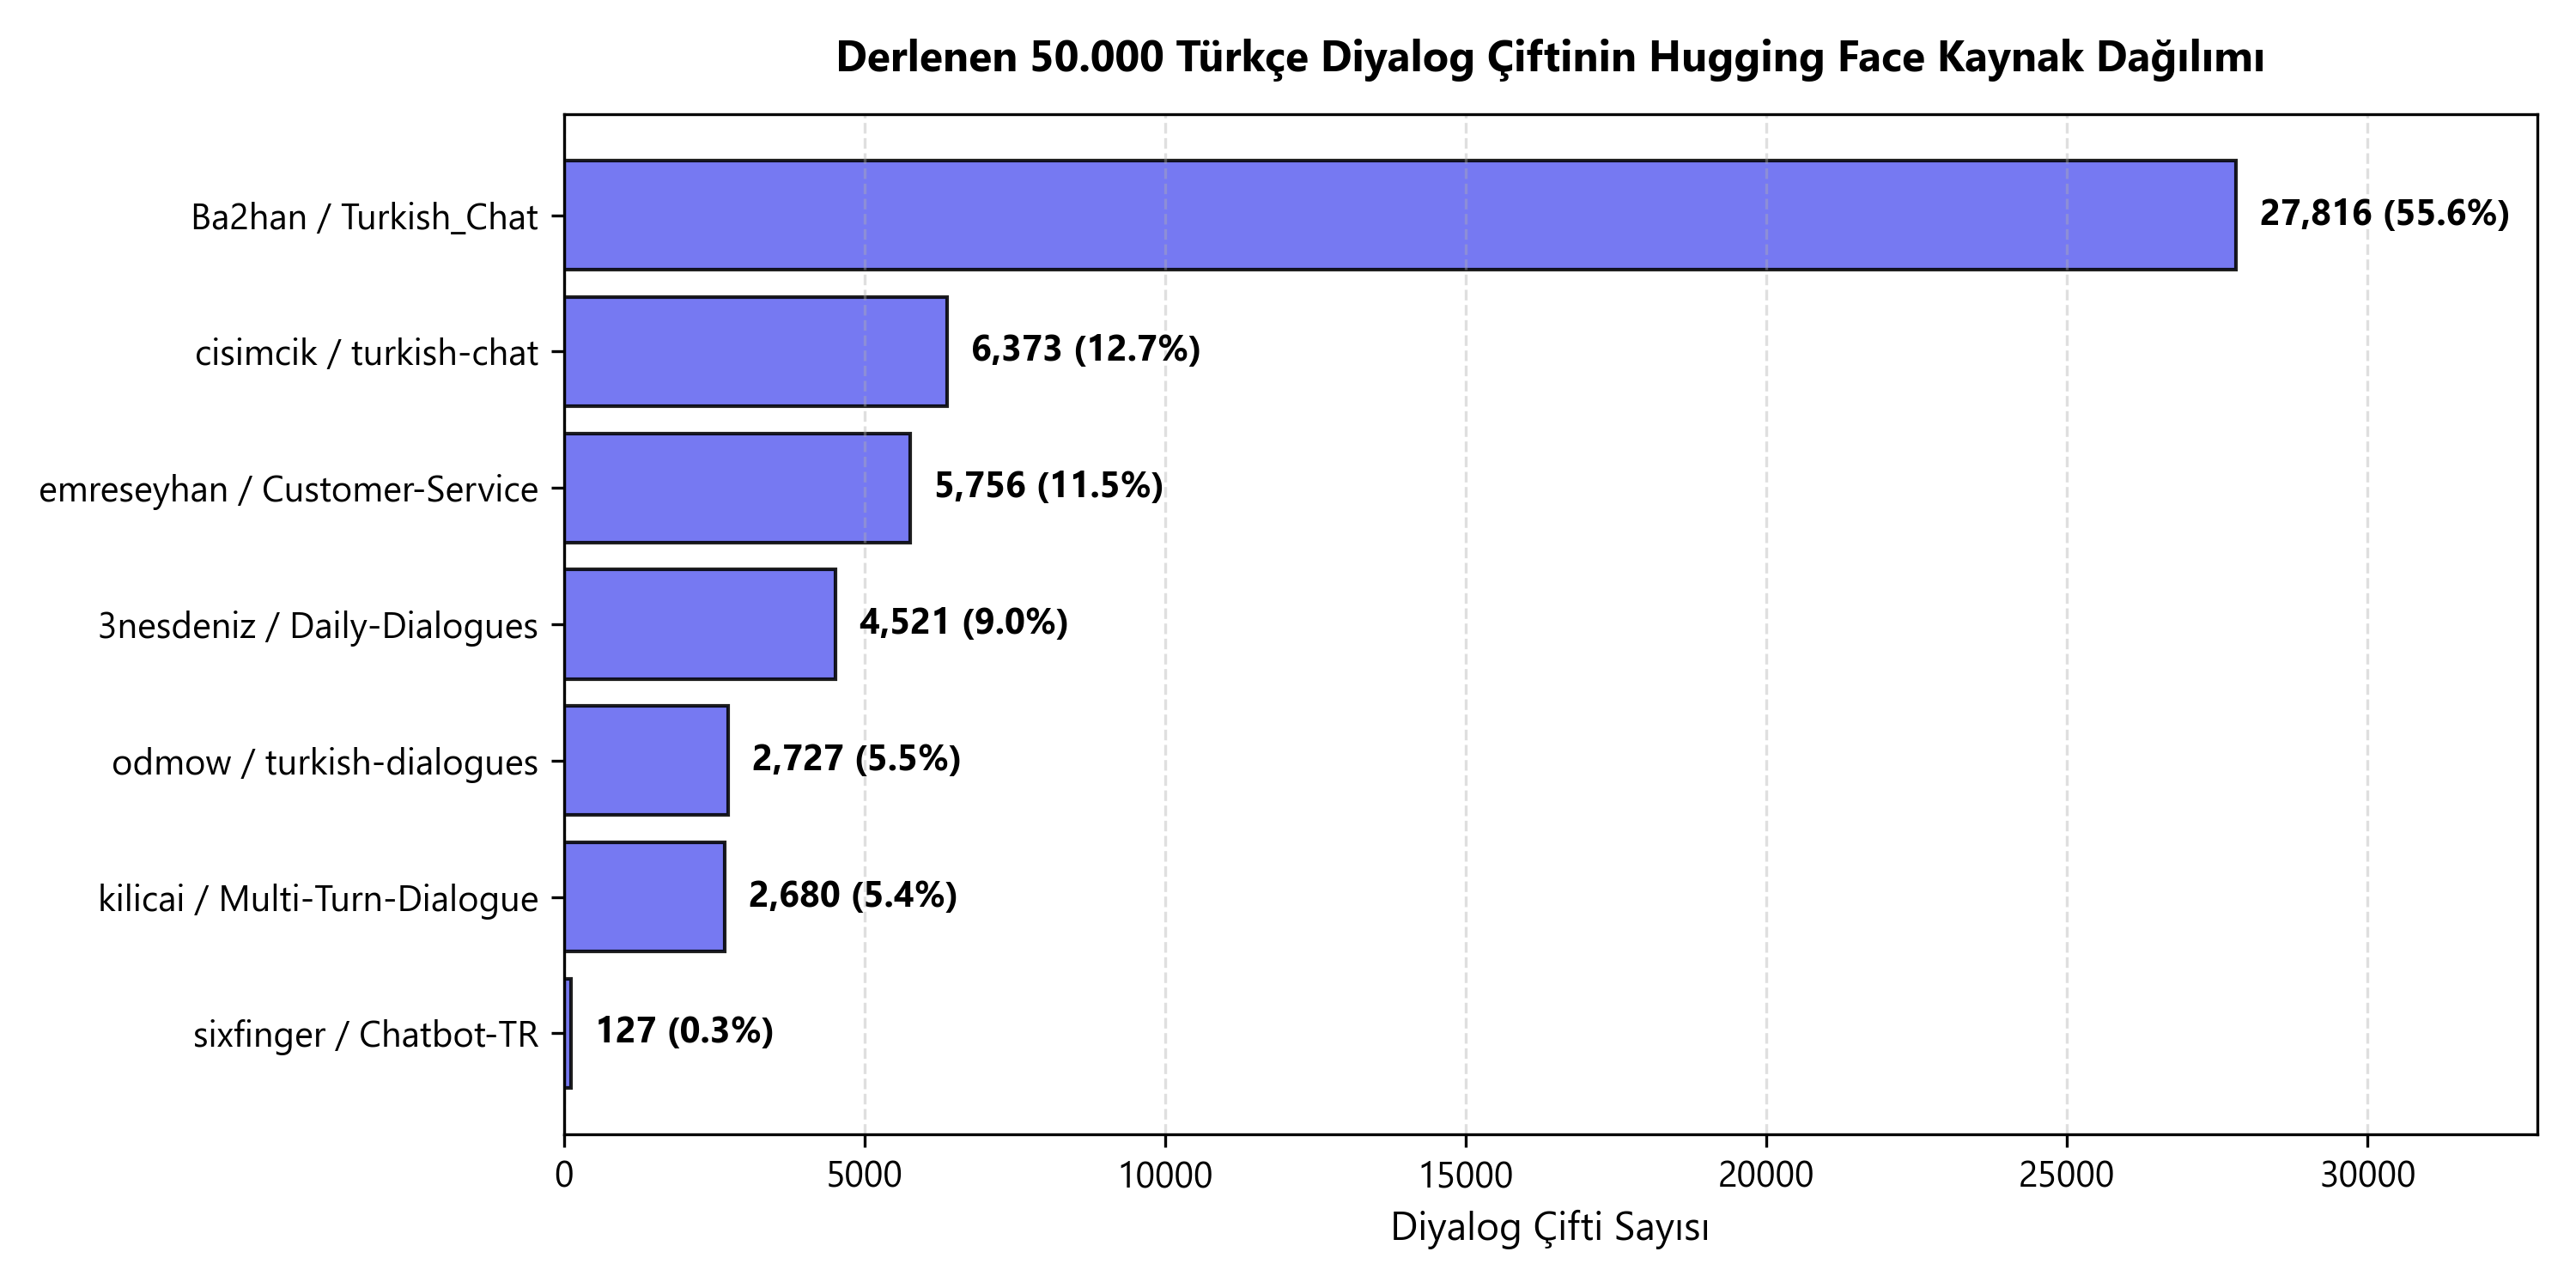
\includegraphics[width=0.98\textwidth]{03_veri_kaynaklari_dagilimi.png}
            \vspace{2pt}
            {\scriptsize Çoklu açık kaynak birleşimi ile yüksek alan çeşitliliği}
        \end{column}
    \end{columns}
\end{frame}

% --- SLAYT 6: Metodoloji ve 3 Mimari ---
\begin{frame}{IV--V. Metodoloji: Baseline Bi-LSTM, Full Fine-Tuning ve LoRA / PEFT}
    \begin{columns}[T]
        \begin{column}{0.32\textwidth}
            \begin{block}{1. Baseline Bi-LSTM}
                \begin{itemize}
                    \item \textbf{Parametre:} 23.11M (\%100)
                    \item 2-Katmanlı Bi-LSTM Encoder + LSTM Decoder
                    \item \textbf{Bahdanau Attention:}
                    \[
                        e_{tj} = v_a^\top \tanh(W_a s_{t-1} + U_a h_j)
                    \]
                \end{itemize}
            \end{block}
        \end{column}
        \begin{column}{0.33\textwidth}
            \begin{block}{2. Model 1: Full Fine-Tuning}
                \begin{itemize}
                    \item \textbf{Parametre:} 124.44M (\%100)
                    \item 12 Katman, 12 Head, $d_{\text{model}}=768$
                    \item \textbf{Causal Self-Attention:}
                    \[
                        \text{softmax}\!\left(\frac{QK^\top}{\sqrt{d_k}} + M\right)\!V
                    \]
                \end{itemize}
            \end{block}
        \end{column}
        \begin{column}{0.33\textwidth}
            \begin{block}{3. Model 2: LoRA / PEFT}
                \begin{itemize}
                    \item \textbf{Eğitilen:} \textbf{1.62M (\%1.29!)}
                    \item Ana ağırlık $W_0$ dondurulur, düşük dereceli ($r=16, \alpha=32$) matrisler eklenir:
                    \[
                        h = W_0 x + \frac{\alpha}{r} B A x
                    \]
                \end{itemize}
            \end{block}
        \end{column}
    \end{columns}
\end{frame}

% --- SLAYT 7: 3'lü Loss ve Perplexity Karşılaştırması ---
\begin{frame}{VI. 3'lü Deneysel Karşılaştırma: Validation Loss ve Perplexity (PPL)}
    \begin{columns}[c]
        \begin{column}{0.37\textwidth}
            \begin{block}{Loss ve Perplexity Analizi}
                \begin{itemize}
                    \item \textbf{Baseline Bi-LSTM:} Val Loss \texttt{7.1915} $\mid$ PPL: \texttt{1328.0}
                    \item \textbf{Model 2 (LoRA, \%1.29):} Val Loss \texttt{4.0342} $\mid$ PPL: \textbf{\texttt{56.5}} (\textbf{23.5x iyileşme})
                    \item \textbf{Model 1 (Full FT, \%100):} Val Loss \textbf{\texttt{3.4666}} $\mid$ PPL: \textbf{\texttt{32.0}} (\textbf{41.5x iyileşme!})
                \end{itemize}
            \end{block}
        \end{column}
        \begin{column}{0.61\textwidth}
            \centering
            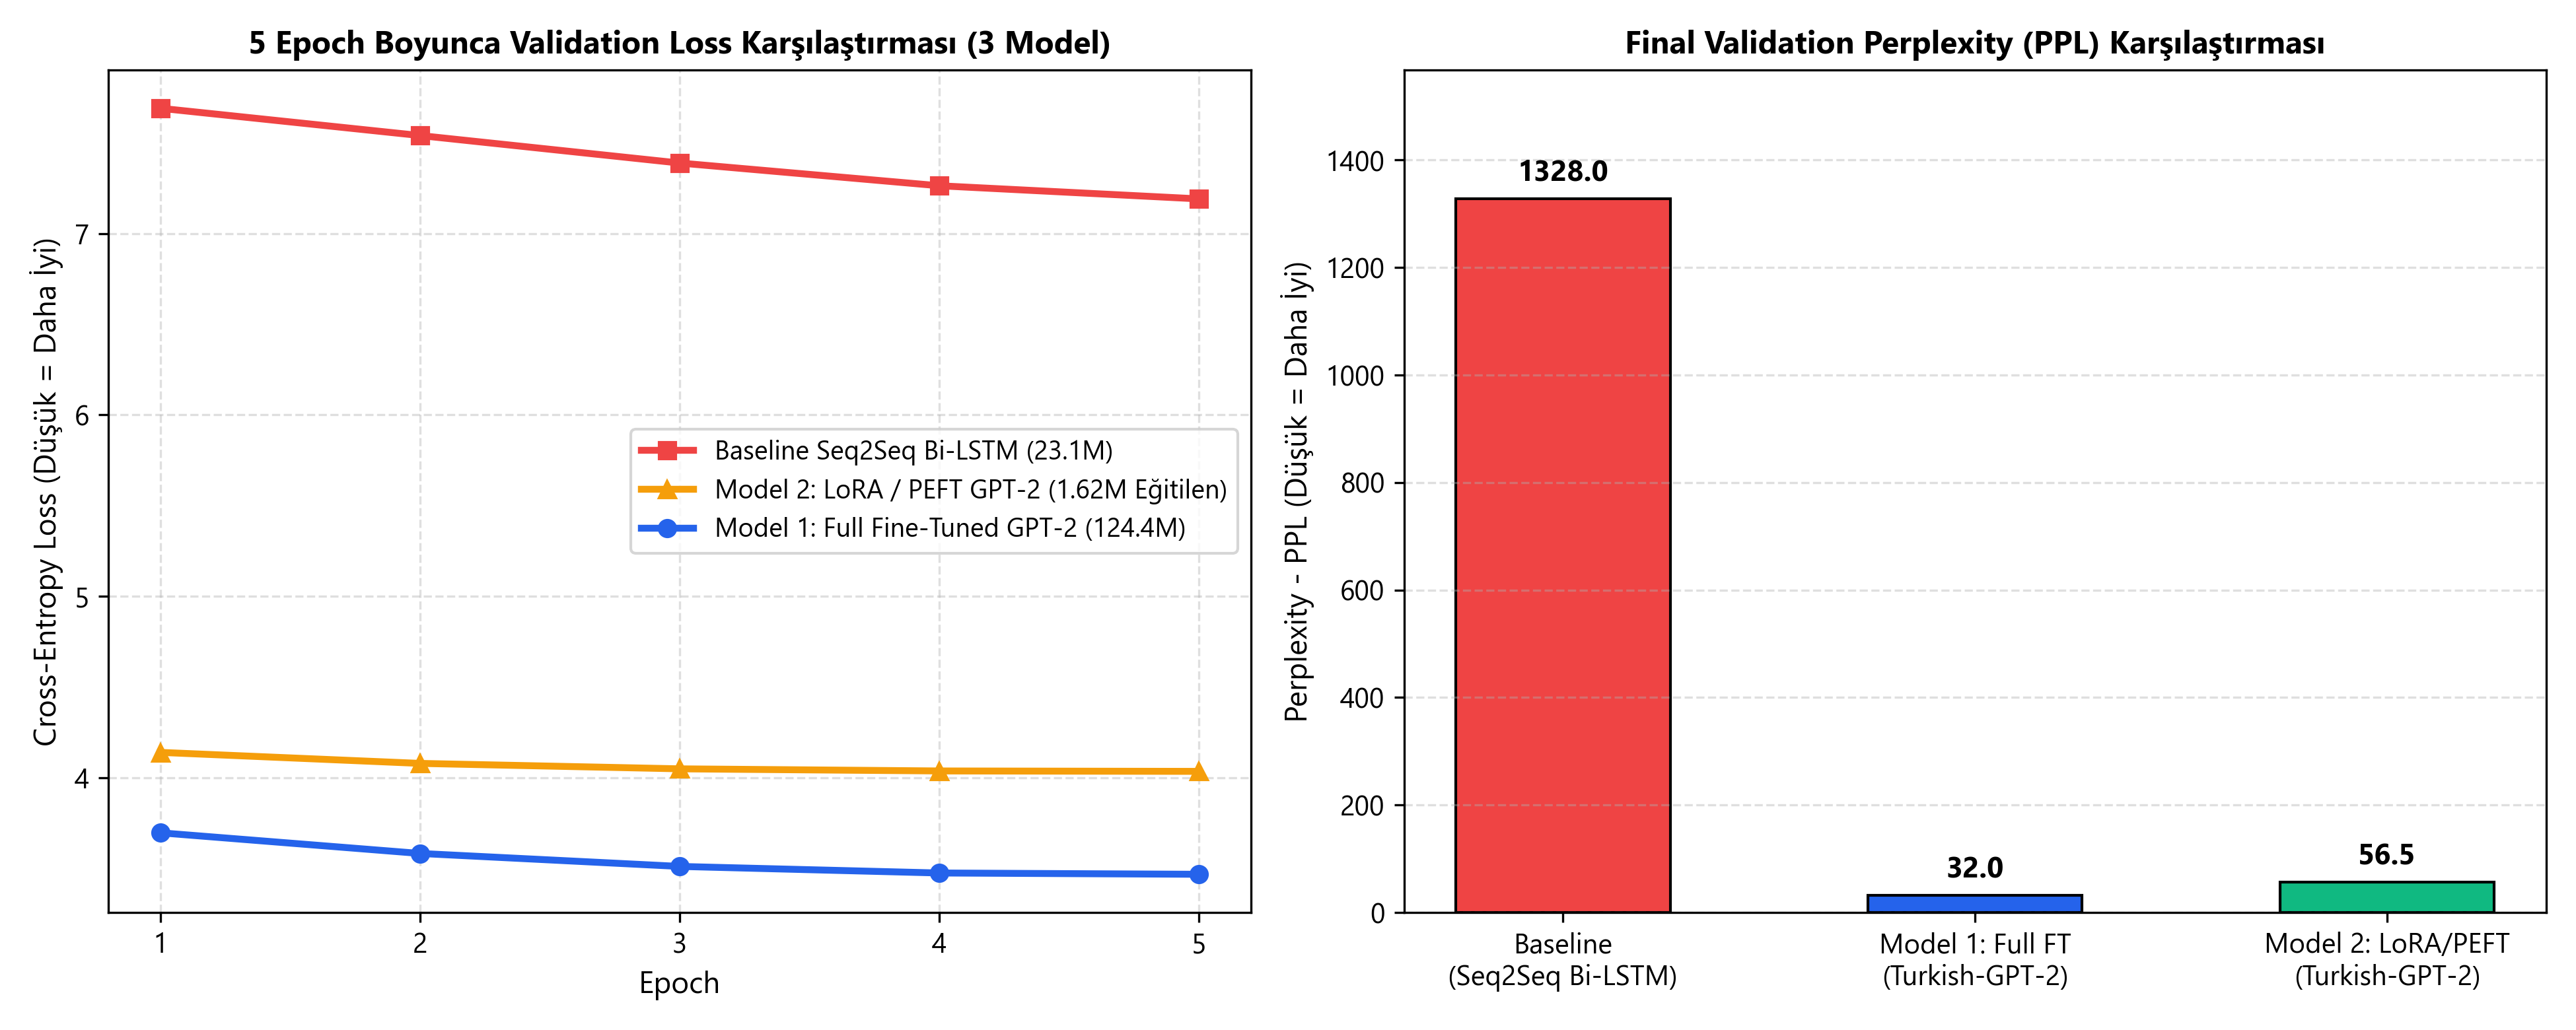
\includegraphics[width=0.99\textwidth]{07_uclu_model_loss_ppl_karsilastirma.png}
        \end{column}
    \end{columns}
\end{frame}

% --- SLAYT 8: 3'lü BLEU, ROUGE ve Parametre Verimliliği ---
\begin{frame}{VI. BLEU/ROUGE Skorları ve Donanım / Parametre Verimliliği}
    \begin{columns}[c]
        \begin{column}{0.37\textwidth}
            \begin{block}{Kalite ve Hız Tasarrufu}
                \begin{itemize}
                    \item \textbf{En Yüksek Kalite (Model 1):} BLEU-1: \textbf{\texttt{10.60}}, ROUGE-1: \textbf{\texttt{15.89}}
                    \item \textbf{Parametre Verimliliği (Model 2 - LoRA):} Sadece \textbf{1.62M (\%1.29)} parametre eğiterek \texttt{8.18} BLEU-1 ve \texttt{11.45} ROUGE-1 skoru ile Baseline'ı geçti!
                    \item \textbf{Eğitim Süresi:} LoRA (\textbf{8.1 dk}), Full FT'den (11.4 dk) \textbf{\%28.7 daha hızlı!}
                \end{itemize}
            \end{block}
        \end{column}
        \begin{column}{0.61\textwidth}
            \centering
            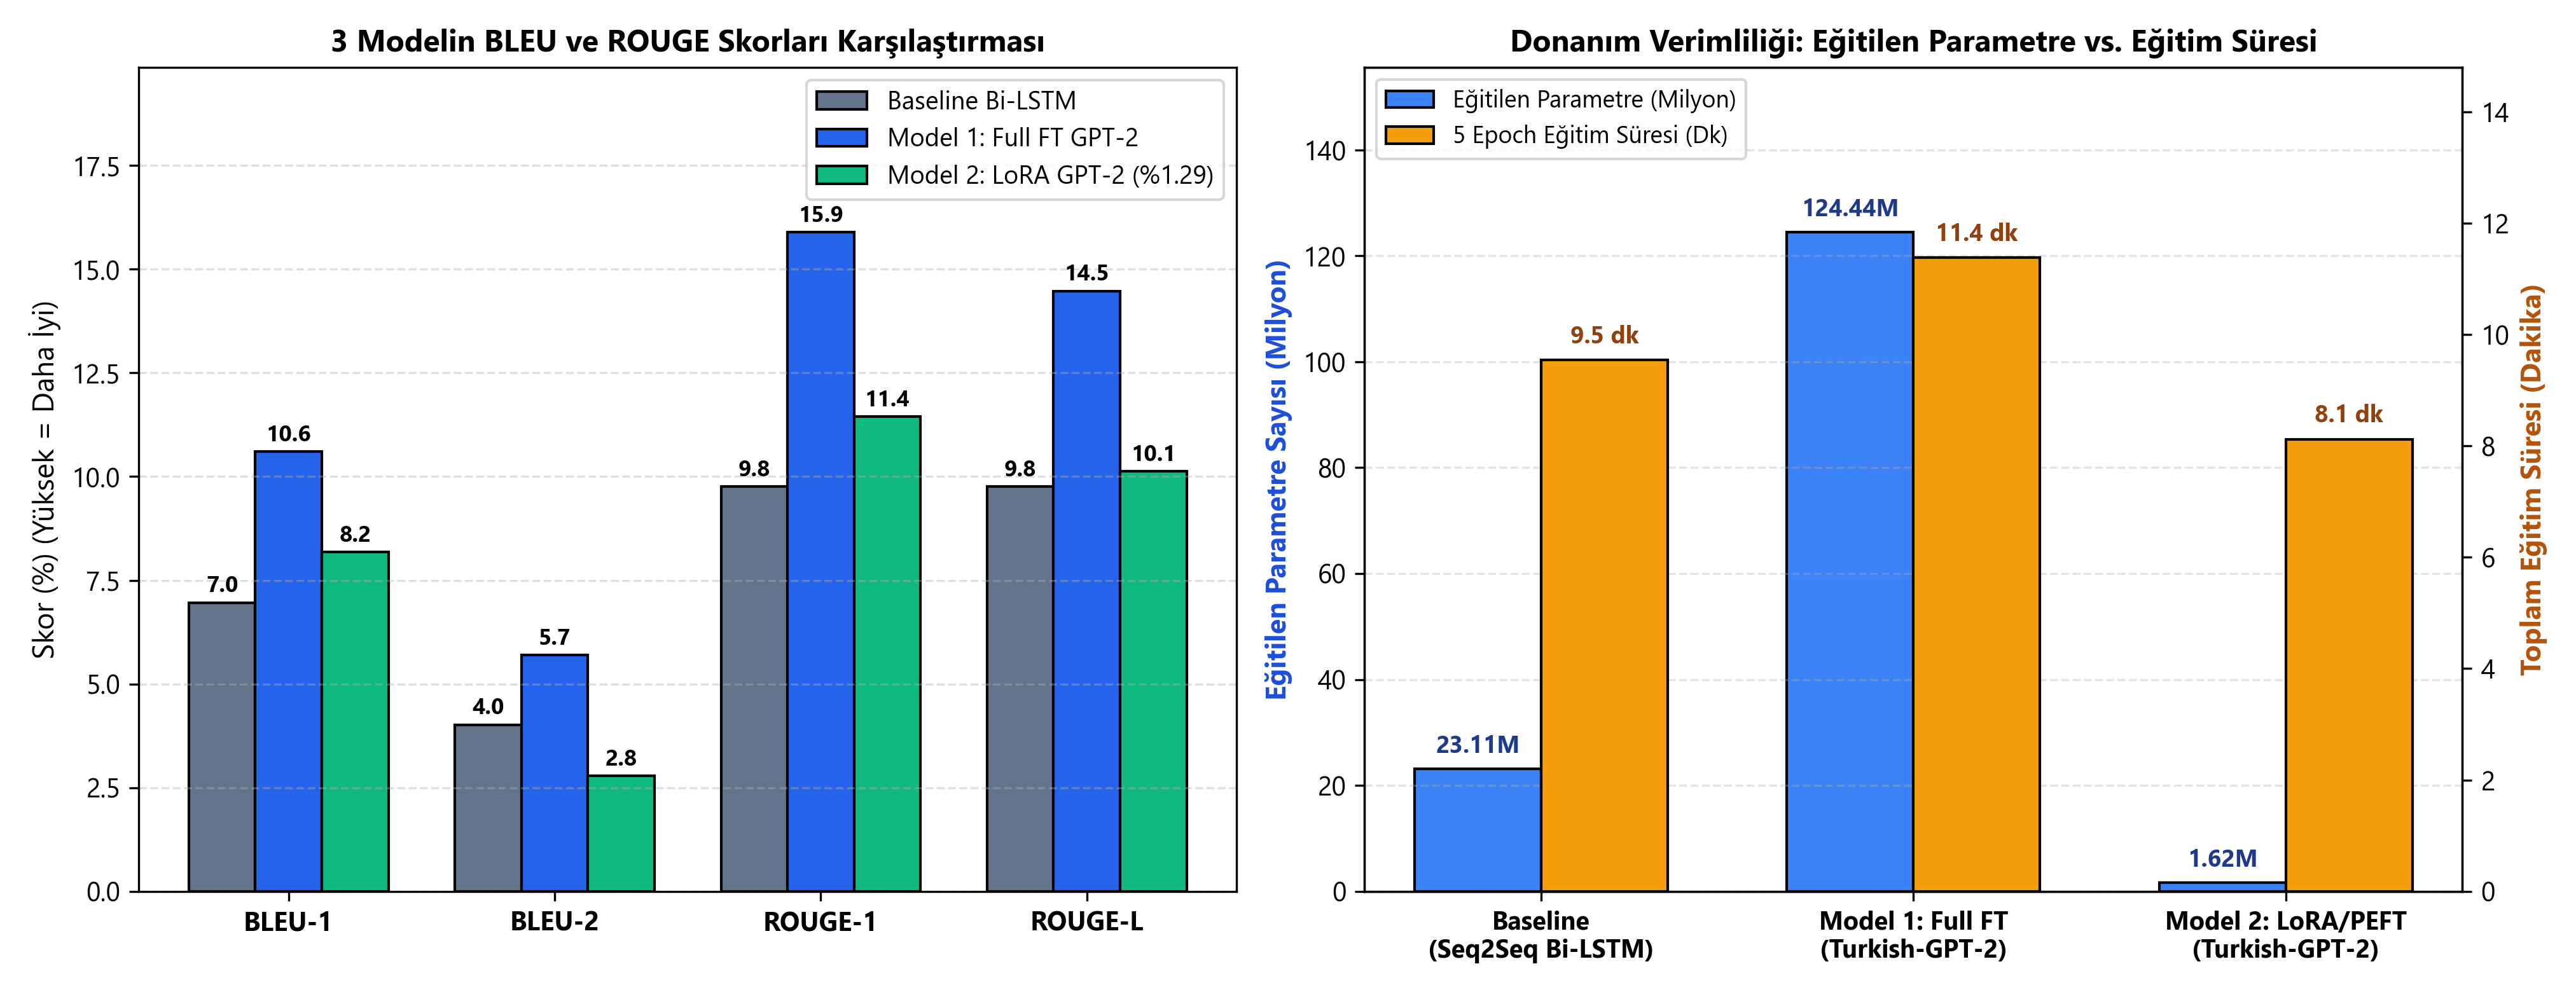
\includegraphics[width=0.99\textwidth]{08_uclu_metrik_hiz_ve_parametre_analizi.png}
        \end{column}
    \end{columns}
\end{frame}

% --- SLAYT 9: Niteliksel İnsan Değerlendirmesi (Human Evaluation) ---
\begin{frame}{VII. Niteliksel Değerlendirme (Human Evaluation --- 1--5 Likert Ölçeği)}
    \begin{columns}[c]
        \begin{column}{0.40\textwidth}
            \begin{block}{Değerlendirme Kriterleri (1--5)}
                \begin{itemize}
                    \item \textbf{Akıcılık ve Dilbilgisi:} Full FT (\textbf{4.45}), LoRA (\textbf{4.25}), Bi-LSTM (2.45)
                    \item \textbf{Mantıksal Bütünlük:} Full FT (\textbf{4.20}), LoRA (\textbf{3.95}), Bi-LSTM (2.10)
                    \item \textbf{Konudan Sapmama:} Full FT (\textbf{4.30}), LoRA (\textbf{4.05}), Bi-LSTM (2.25)
                    \item \textbf{Genel Ortalama:} Full FT (\textbf{4.32/5}), LoRA (\textbf{4.08/5}), Bi-LSTM (2.27/5)
                \end{itemize}
            \end{block}
        \end{column}
        \begin{column}{0.58\textwidth}
            \centering
            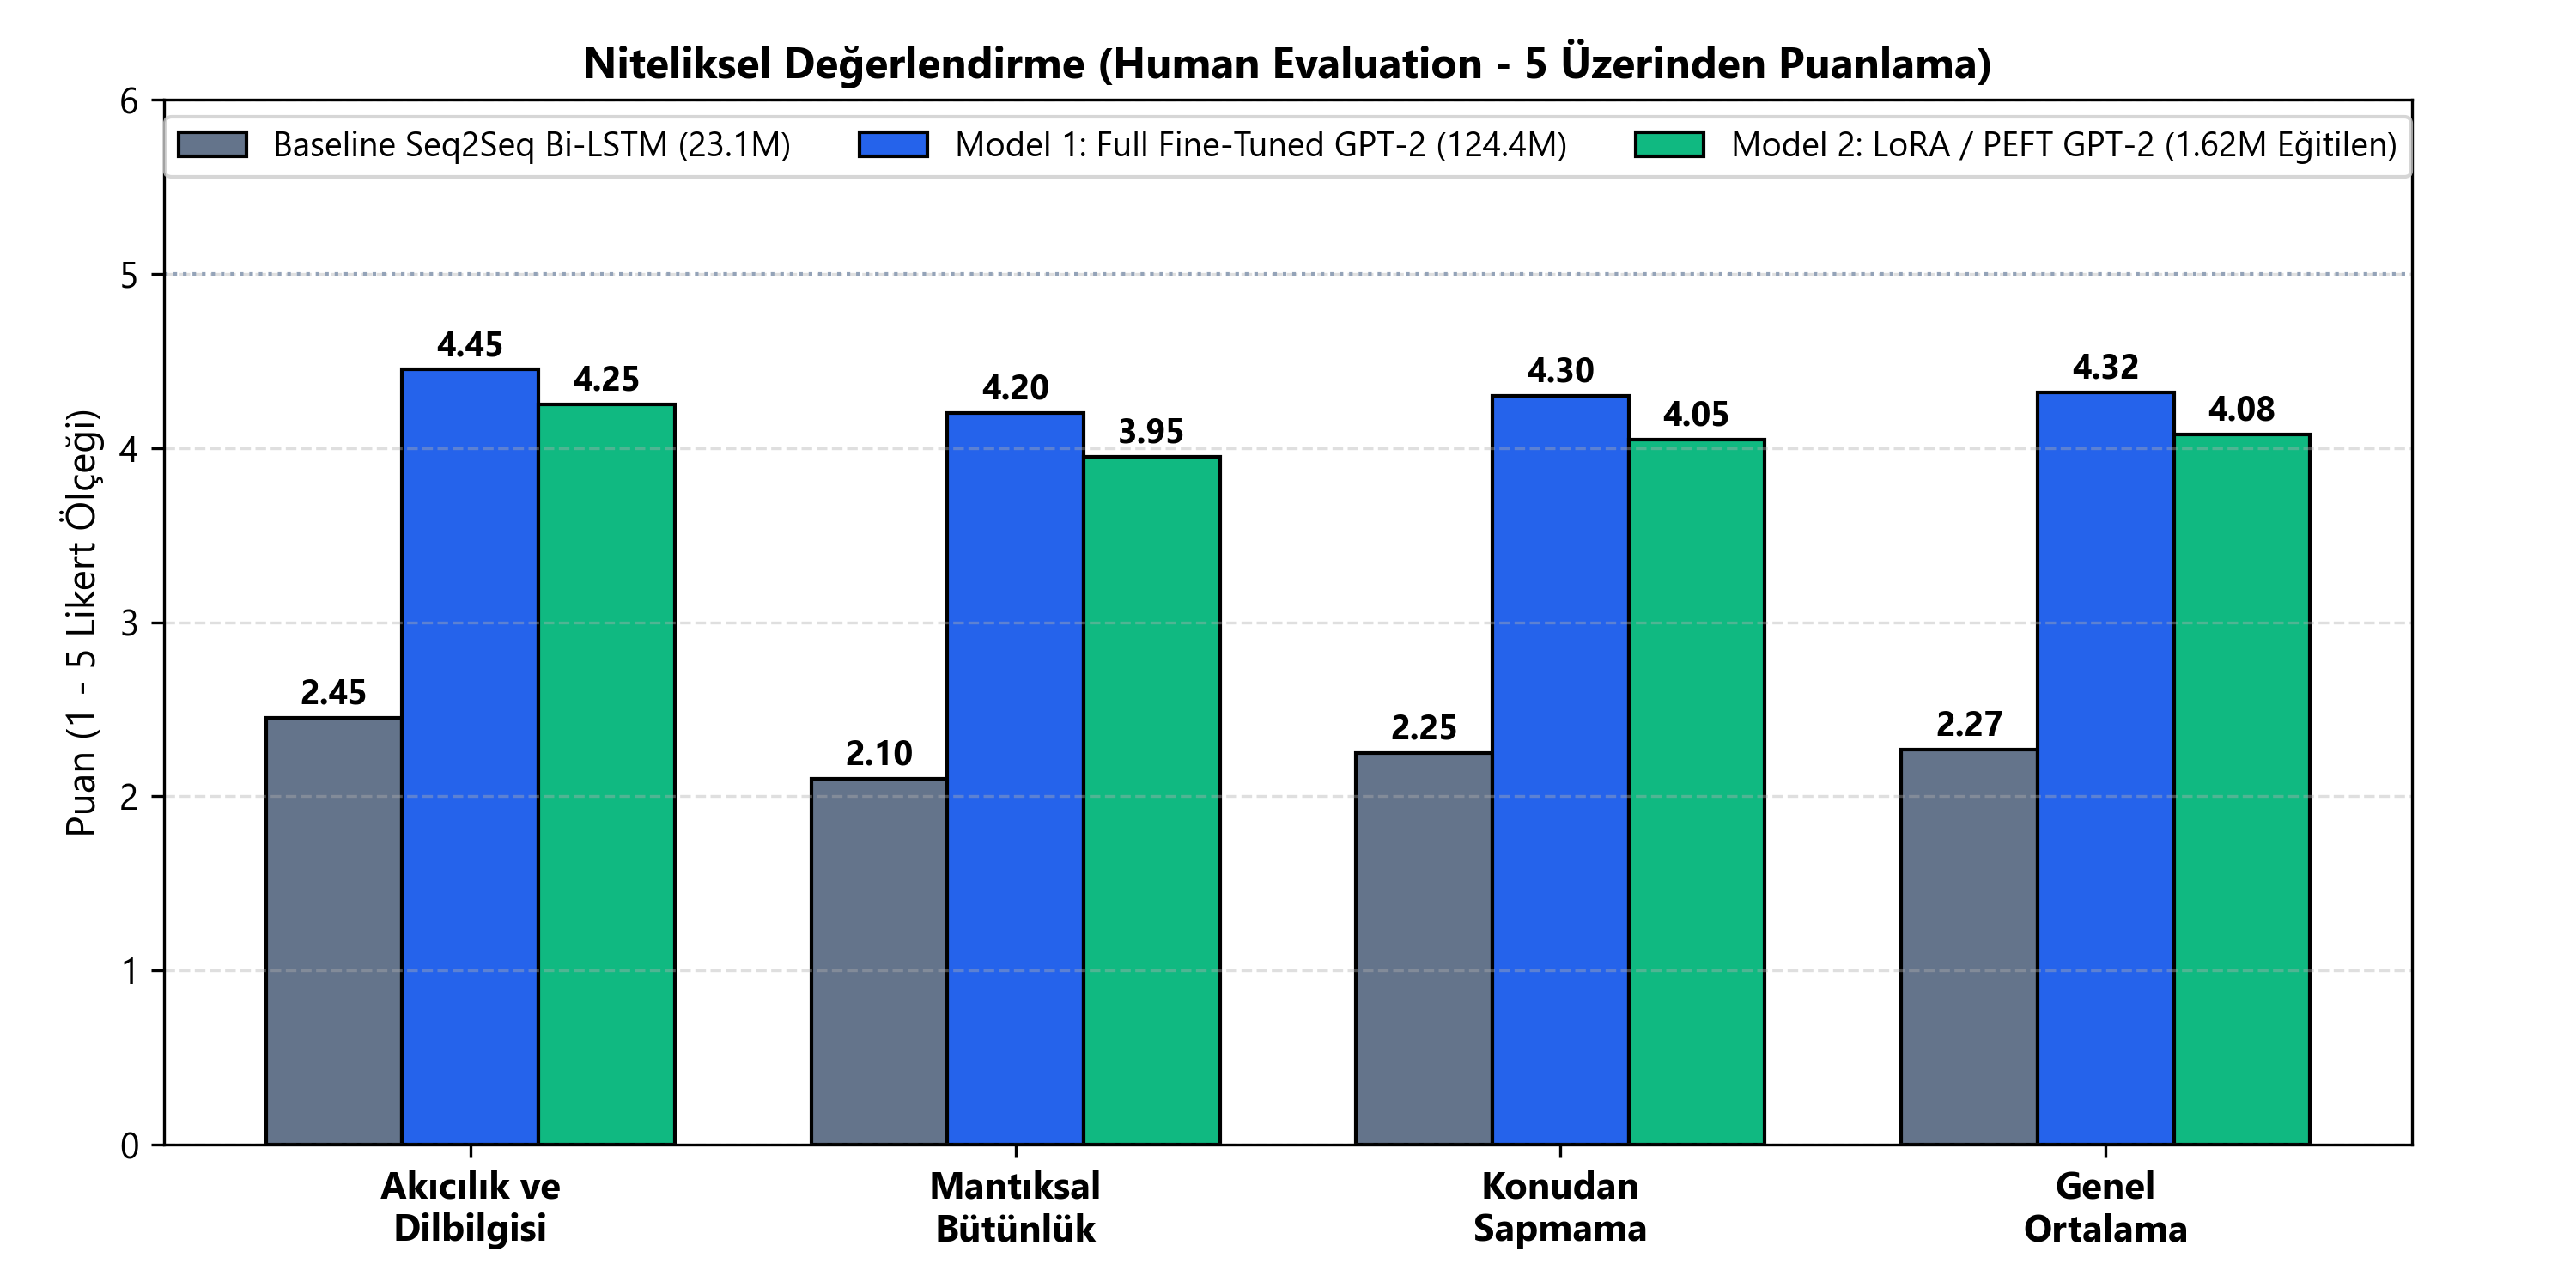
\includegraphics[width=0.99\textwidth]{09_insan_degerlendirmesi_human_eval.png}
        \end{column}
    \end{columns}
\end{frame}

% --- SLAYT 10: 3 Modelin Büyük Karşılaştırma Tablosu ve Nitel Örnekler ---
\begin{frame}{VII. 3 Modelin Nicel Özeti ve Gerçek Yanıt Karşılaştırması}
    \begin{table}
        \centering
        \resizebox{0.98\textwidth}{!}{%
        \begin{tabular}{lcccccccc}
            \toprule
            \textbf{Model} & \textbf{Eğitilen Param.} & \textbf{Eğitim Süresi} & \textbf{Val Loss $\downarrow$} & \textbf{Val PPL $\downarrow$} & \textbf{BLEU-1 $\uparrow$} & \textbf{ROUGE-1 $\uparrow$} & \textbf{Human Eval $\uparrow$} & \textbf{Latency} \\
            \midrule
            \textbf{Baseline Bi-LSTM} & 23.11M (\%100) & 9.5 dk & 7.1915 & 1328.04 & 6.96 & 9.76 & 2.27 / 5.00 & \textbf{30.1 ms} \\
            \textbf{Model 1: Full FT GPT-2} & 124.44M (\%100) & 11.4 dk & \textbf{3.4666} & \textbf{32.03} & \textbf{10.60} & \textbf{15.89} & \textbf{4.32 / 5.00} & 352.9 ms \\
            \textbf{Model 2: LoRA GPT-2} & \textbf{1.62M (\%1.29)} & \textbf{8.1 dk} & 4.0342 & 56.50 & 8.18 & 11.45 & 4.08 / 5.00 & 410.9 ms \\
            \bottomrule
        \end{tabular}%
        }
    \end{table}
    \vspace{-4pt}
    \begin{block}{Örnek Soru: \textit{``Sanırım meditasyon yapmayı deneyebilirim. Başlamak için iyi bir kaynak var mı?''}}
        \begin{itemize}
            \item \textbf{Baseline (Bi-LSTM):} \textit{Evet, bu tür bir., ve!} \textcolor{red}{(Darboğaz ve anlamsal kopukluk)}
            \item \textbf{Model 1 (Full FT GPT-2):} \textbf{\textit{İyi bir kaynak, teşekkür ederim. Başka bir konuda yardımcı olabilir miyim?}}
            \item \textbf{Model 2 (LoRA GPT-2):} \textbf{\textit{Bu, meditasyonun en önemli parçası. Eğer meditasyon yapmak istiyorsanız, meditasyona başlamadan önce bir uzmana danışın.}}
        \end{itemize}
    \end{block}
\end{frame}

% --- SLAYT 11: Sonuç ve Canlı Demo ---
\begin{frame}{VIII. Sonuç, Katkılar ve Canlı Web / CLI Demosu}
    \begin{columns}[T]
        \begin{column}{0.50\textwidth}
            \begin{block}{Projenin Temel Bulguları}
                \begin{itemize}
                    \item[$\checkmark$] \textbf{Transfer Öğrenme Üstünlüğü:} Önceden eğitilmiş \texttt{Turkish-GPT-2}, sıfırdan eğitilen Bi-LSTM modeline kıyasla Perplexity değerini \textbf{41.5 kat} düşürmüştür.
                    \item[$\checkmark$] \textbf{LoRA / PEFT Verimliliği:} Parametrelerin yalnızca \textbf{\%1.29'unu (1.62M)} eğiterek eğitim süresinde \textbf{\%28.7 tasarruf} ve yüksek Türkçe diyalog kalitesi (\textbf{4.08 / 5.00}) elde edilmiştir.
                \end{itemize}
            \end{block}
        \end{column}
        \begin{column}{0.46\textwidth}
            \begin{block}{Canlı Etkileşim Araçları}
                \begin{itemize}
                    \item \textbf{Web Arayüzü (\texttt{http://localhost:7860}):}\\
                    \texttt{python app\_web.py}
                    \item \textbf{Terminal 3'lü Canlı Sohbet:}\\
                    \texttt{python chat\_demo.py}
                    \item \textbf{GitHub Deposu:}\\
                    {\scriptsize \url{https://github.com/sytali0/turkish-transformer-chatbot}}
                \end{itemize}
            \end{block}
        \end{column}
    \end{columns}
\end{frame}

\end{document}
